\sectiontinyvert{Architecture details} \label{sec:architecture_details}

\begin{figure}[tbh]
\centering
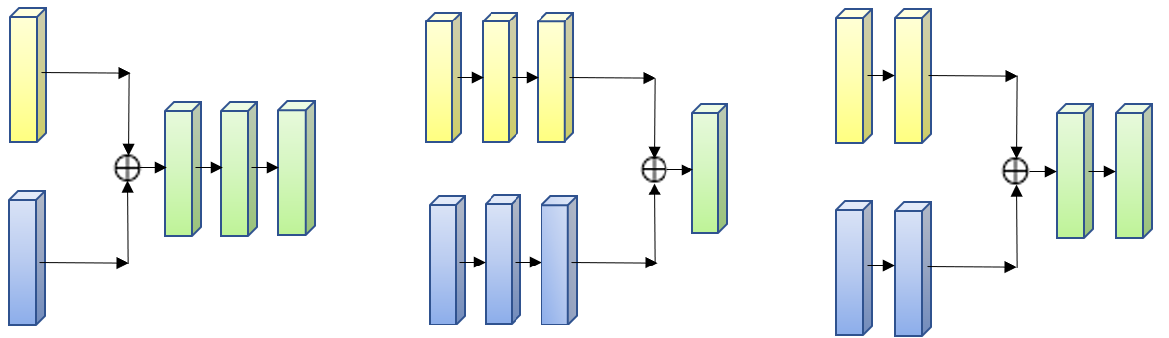
\includegraphics[width=\linewidth]{./images/early_late_middle_fusion.png}
\setlength{\abovecaptionskip}{-10pt plus 3pt minus 2pt}
\setlength{\belowcaptionskip}{-15pt plus 3pt minus 2pt}
\caption{Fusion schemes. Left: early fusion; Middle: late fusion; Right: middle fusion. Yellow and blue blocks symbolize features from distinct input branches, and green blocks represent fused data. Each block stands for a tensor of features. }
\label{fig:fusion}
\end{figure}
\begin{figure*}[!th]
\centering
% \includegraphics[width=\textwidth]{./images/Tech_Details_Transformer.pdf}
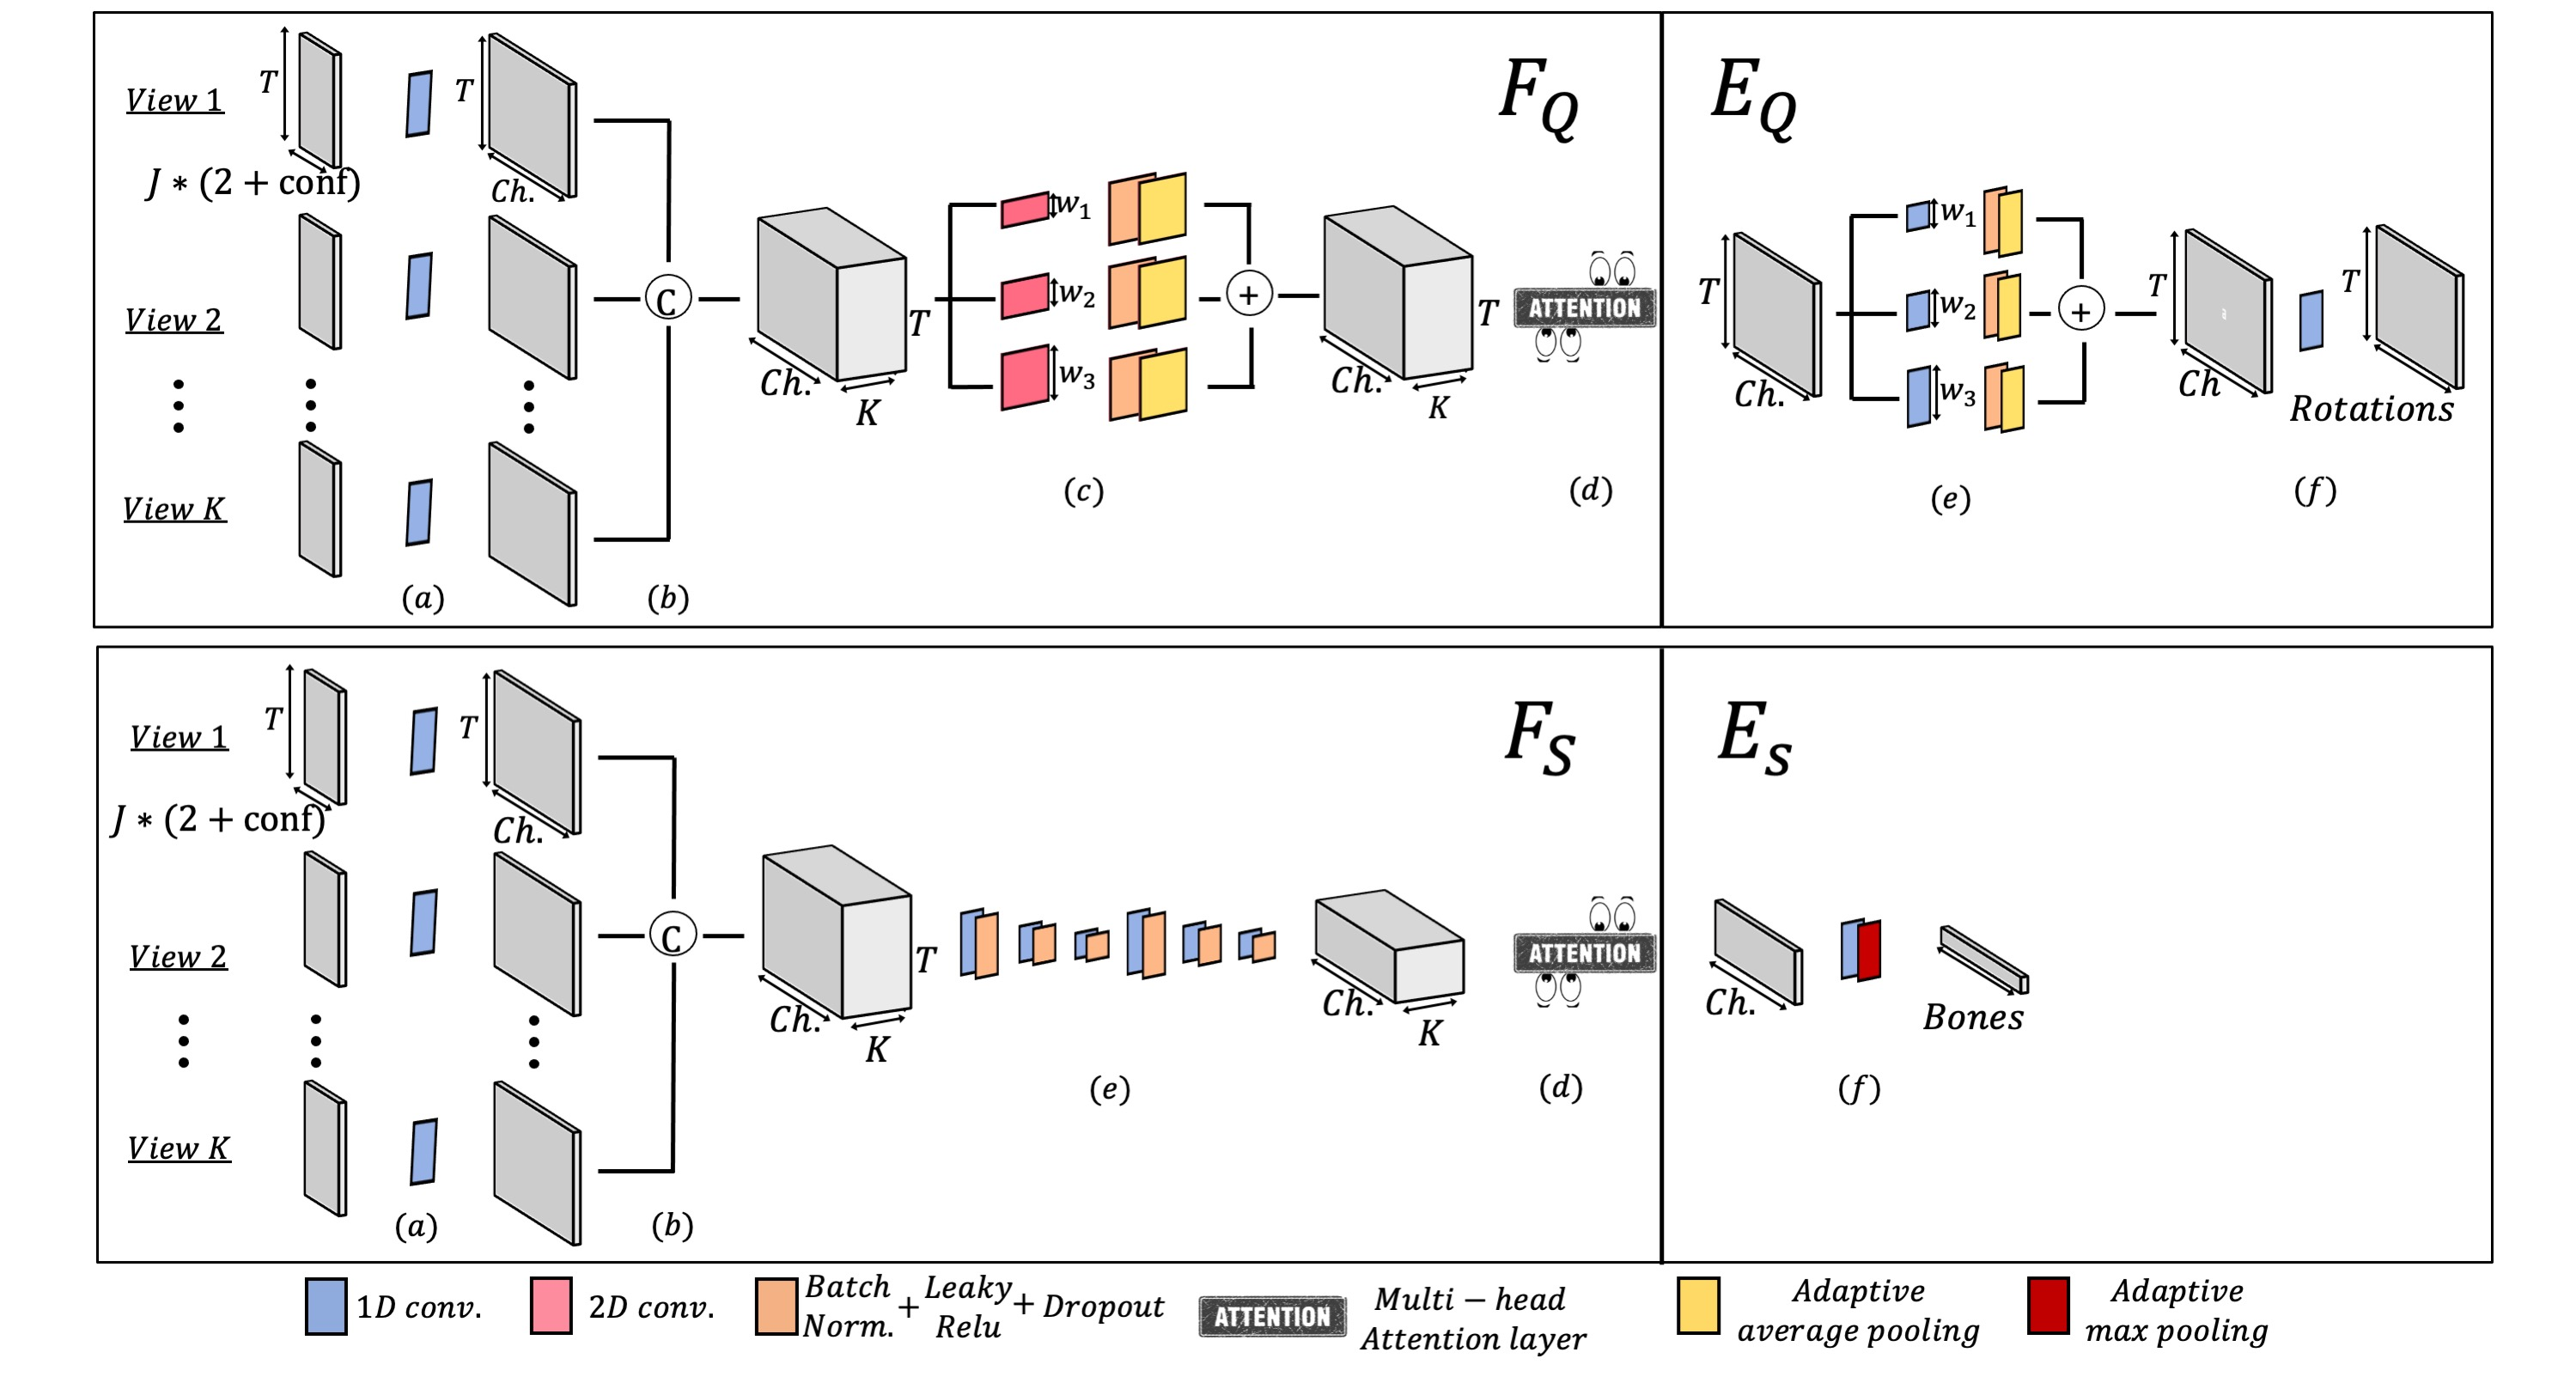
\includegraphics[width=\linewidth]{./images/Tech_Details_MHA.jpg}

\setlength{\abovecaptionskip}{0pt plus 3pt minus 2pt}
\setlength{\belowcaptionskip}{10pt plus 3pt minus 2pt}

\caption{Architecture in detail. The upper and lower parts are the rotations and bones branches, respectively.  (a) Channel-wise expansion layer; (b) View concatenation; (c) Multi-view convolutional filters; (d) Cross-view attention layer \bg{(detailed in \Cref{fig:attention_detail})}; (e) Single-view convolutional filters; (f) Channel-wise shrinkage layer.}
\label{fig:architecture_detail}
\end{figure*}
\begin{figure*}[!th]
\centering
% \includegraphics[width=\textwidth]{./images/Tech_Details_Transformer.pdf}
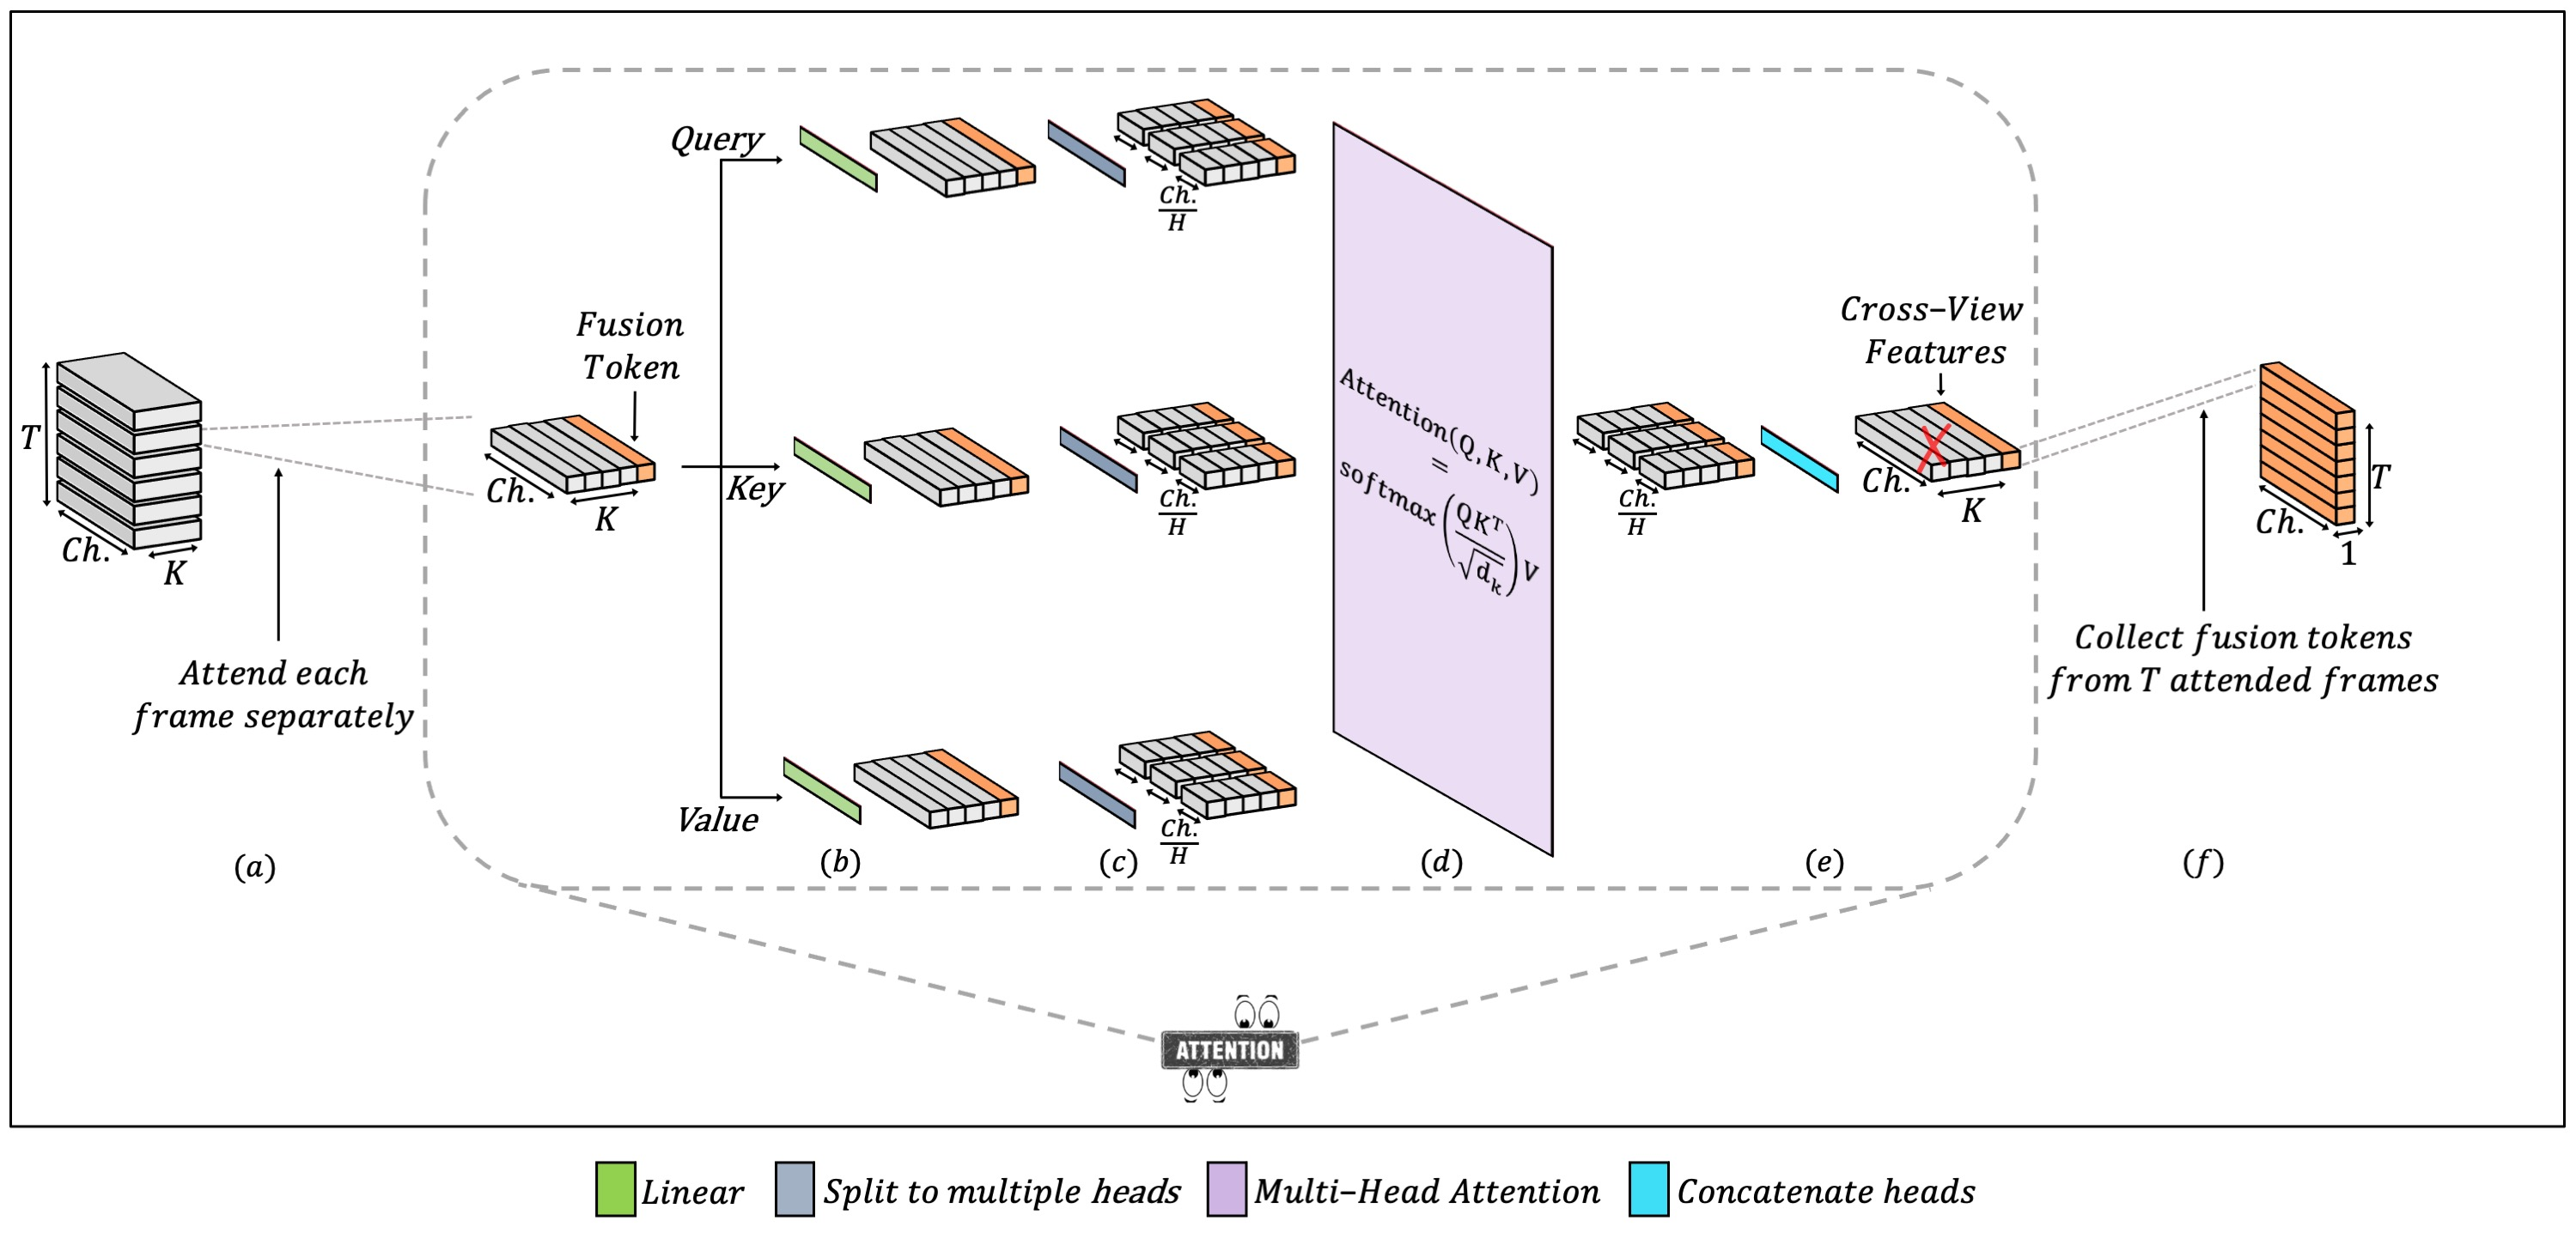
\includegraphics[width=\linewidth]{./images/Attention_diagram.jpg}

\setlength{\abovecaptionskip}{5pt plus 3pt minus 2pt}
\setlength{\belowcaptionskip}{-10pt plus 3pt minus 2pt}
\caption{\bg{Cross-view attention layer (\Cref{fig:architecture_detail}(d)) in detail. Our attention mechanism processes each frame separately, attending the multi-view features and fusing them to a single output per frame. 
(a)~Process each temporal frame independently. Add a learned token~\cite{BERT} that forms a \emph{fusion view}; 
%A learned fusion token is added to multi-view .... , similar approach as Devlin~\etal\cite{BERT}; 
(b)~Linear layer; 
(c)~Split the channels to $H$ attention heads; 
(d)~Multi-Head attention~\cite{attn_is_all_you_need}; 
(e)~Concatenate the attention heads; 
(f)~Drop features from the original views. Collect fusion view features from all the frames in the temporal sequence. }}
\label{fig:attention_detail}
\end{figure*}
\begin{table*}[bht]
\setlength{\abovecaptionskip}{5pt plus 3pt minus 2pt}
\setlength{\belowcaptionskip}{0pt plus 3pt minus 2pt}
\caption{FLEX structure. $\bJ$ denotes the number of joints, $\bK$ the number of views, and $\bL$ denotes the number of limbs. $k$ and $s$ denote kernel width and the stride, respectively. $\rightarrow$ denotes parallel convolutions while $\downarrow$ denotes sequential ones.}
\resizebox{\textwidth}{!}{
\begin{tabular}{| l | c | l | c | c | c |}
\hline
\toprule
Name & & Layers & $k$ & $s$ & in\; /\; out \\
\hline
\midrule %motion encoder 
$F_Q$  & &1D-Conv + BatchNorm + LReLU + Dropout  & $1$ & 1 & $3J\; /\; 1024$\\
\cline{2-5}
& $\rightarrow$ &2D-Conv + BatchNorm + LReLU + Dropout + Adap AP & $5$ & 3 & $1024\; /\; 1024$\\
& $\rightarrow$ &2D-Conv + BatchNorm + LReLU + Dropout + Adap AP & $3$ & 1 & $1024\; /\; 1024$\\
& $\rightarrow$ &2D-Conv + BatchNorm + LReLU + Dropout + Adap AP & $1$ & 1 & $1024\; /\; 1024$\\
\cline{2-5}
% & &Transformer Encoder (2 attention heads) & $1$ & 1 & $1024\; /\; 1024$\\
% & &Transformer Encoder (2 attention heads) & $1$ & 1 & $1024\; /\; 1024$\\
& & Multi-head Attention layer (64 heads) & $-$ & $-$ & $1024\; /\; 1024$\\

\hline
$E_Q$ & $\rightarrow$ &1D-Conv + BatchNorm + LReLU + Dropout + Adap AP & $5$ & 3 & $1024\; /\; 1024$\\
& $\rightarrow$ &1D-Conv + BatchNorm + LReLU + Dropout + Adap AP & $3$ & 1 & $1024\; /\; 1024$\\
& $\rightarrow$ &1D-Conv + BatchNorm + LReLU + Dropout + Adap AP & $1$ & 1 & $1024\; /\; 1024$\\
\cline{2-5}
& & 1D-Conv & $1$ & 1 & $1024 / 4(J\!-\!1)\!+\!4K$\\
\hline
\midrule %body encoder
$D$ & & 1D-Conv + ReLU  & $1$ & 1 & $4J \; /\; 1024$\\
& $\downarrow$&1D-Conv + ReLU + Adap AP & $1$ & 1 & $1024\; /\; 24J$\\
& &Linear & $-$ & $-$ & $24J \; /\; J$\\
\hline
\midrule %body encoder
$F_S$ & & 1D-Conv + BatchNorm + LReLU + Dropout  & $1$ & 1 & $J3\; /\; 1024$\\
\cline{2-5}
& &1D-Conv + BatchNorm + LReLU + Dropout & $5$ & 1 & $1024\; /\; 1024$\\
& $\downarrow$ &1D-Conv + BatchNorm + LReLU + Dropout & $3$ & 1 & $1024\; /\; 1024$\\
& &1D-Conv + BatchNorm + LReLU + Dropout & $1$ & 1 & $1024\; /\; 1024$\\
\cline{2-5}
& &1D-Conv + BatchNorm + LReLU + Dropout & $5$ & 1 & $1024\; /\; 1024$\\
& $\downarrow$ &1D-Conv + BatchNorm + LReLU + Dropout & $3$ & 1 & $1024\; /\; 1024$\\
& &1D-Conv + BatchNorm + LReLU + Dropout & $1$ & 1 & $1024\; /\; 1024$\\
\cline{2-5}
% & &Transformer Encoder (2 attention heads) & $1$ & 1 & $1024\; /\; 1024$\\
% & &Transformer Encoder (2 attention heads) & $1$ & 1 & $1024\; /\; 1024$\\
& & Multi-head Attention layer (64 heads) & $-$ & $-$ & $1024\; /\; 1024$\\

\hline
$E_S$ & &Adaptive MP & $-$ & $-$ & $-$\\
& &1D-Conv & $1$ & 1 & $1024\; /\; L$\\
\hline
\bottomrule
\end{tabular}
} % end resizebox
\setlength{\abovecaptionskip}{0pt plus 3pt minus 2pt}
\setlength{\belowcaptionskip}{-20pt plus 3pt minus 2pt}
\caption*{}
\label{tab:layer_detail}
\end{table*}

The architectural blocks in our implementation are the multi-view feature fusion layers $F_S$ and $F_Q$, the two encoders, $E_S$ and $E_Q$, a forward kinematics layer $FK$ and a discriminator $D$.
Our discriminator $D$ is a linear component that contains two convolution layers and one fully connected layer. We base it on Kanazawa~\etal~\shortcite{Kanazawa:2018}). 
%Its output value is between 0 and 1.
The $FK$ layer is based on Villegas \etal~\shortcite{Villegas:2018}. 

There are two novel building blocks contained in the new fusion layers, $F_S$ and $F_Q$. The first is a multi-view convolutional layer; that is, a convolution that is aware of features stemming from  multiple views as well as multiple frames. This convolutional layer is used in $F_Q$ only.
The second is a multi-head attention layer, used in both $F_S$ and $F_Q$.
\sr{A standard attention mechanism looks at the data as a \emph{sequence} of \emph{embeddings}. In our mechanism, the \emph{views} form the sequence, and the \emph{channels} form the embeddings.}
Our attention layer is based on the LiftFormer~\cite{llopart2020liftformer}. While the LiftFormer attends to time, we attend to views. 
\sr{The embedding size is 1024, and we use 64 heads (see \Cref{tab:layer_detail}), so for the Query, Key and Value (each), we have 64 learned linear filters of size $K\times 16$, where $K$ is the number of views and 16 is the result of 1024/64.}


A key architectural choice in our fusion layers, $F_S$ and $F_Q$, is at which stage to fuse the input views. In \Cref{fig:fusion} we depict the conceptual idea of fusing. Each fusing scheme has its own advantages and disadvantages. Following the insight that early convolutional layers yield coarse features and late ones yield semantic features, we observe early fusion as generating all features (coarse and semantic) when a network is aware to all input branches, and observe middle fusion as first generating coarse features that are distinct for each branch, and only then fuse the coarse features together to generate common semantic features. When applying late fusion, the network creates distinct coarse and semantic features for each branch and only then fuses them together.
During the development of our model, we have experimented with different fusion schemes, and found out that for our setting the early fusion works best.

\Cref{fig:architecture_detail} depicts diagrams of the multi-view fusion layers and the encoders. The input to both fusion layers is $\bV_{s,q,r}\in\bbr^{T\times 3J\times K}$ (described in \ifappendix{\Cref{sec:architecture}}\else{the Architecture section of the main paper})\fi. 
In order to make the diagram more intuitive, we sketch $V$ as $K$ temporal sequences. 
%Each temporal sequence is a $T\times 3J$ 2D tensor, with data size $T$ and $3J$ channels. 
Each temporal sequence is a 2D tensor, where channels are formed by the joints.
The fusion layer first streams these temporal sequences through an expansion layer, increasing their channel size. 
Next, our fusion layer concatenates the expanded data and obtains a 3D tensor, on which it applies multi-view convolutional filters. These filters consider the data from all views. At the next stage we apply a multi-head attention layer that attends to views. Our network uses the attention layer output to create a 2D tensor representing one 'fused' view. The features are then passed to the encoder. 
The encoder block $E_Q$ consists of three parallel 1D convolutional layers of different kernel sizes, followed by a final additional 1D convolution. The encoder $E_S$ starts with an adaptive max pooling to collapse the time dimension and then runs a final 1D convolution.
After each convolution block, we apply batch normalization, a leaky rectified linear unit and dropout. 
Finally, we run a shrinking filter to decrease the number of channels to the desired output size. 
Table~\ref{tab:layer_detail} describes the weight parameters of each layer.

\sr{
In \Cref{fig:attention_detail} we zoom into the attention block (item (d) in \Cref{fig:architecture_detail}). 
Each slice of one temporal frame is separately forwarded through this block. 
Such a slice contains features from all the views. Within the attention block, we concatenate an additional view, which we call the \emph{fusion view}. 
This additional view is a learned token~\cite{BERT}, in which the attention mechanism combines significant information from all views. 
Our model attends to all views, including the added one.
After exiting the attention block we omit the data related to the given views and keep the learned fusion view only.
This fusion view is then concatenated with the outputs of the other temporal frames.
}




